\section{Overview}
\paragraph{}Our first sight of the system is from the highest point of view. Here we describe the architecture of the system from a \textit{layer} view.

\subsection{Three-tier-architecture}
We decided to use a \textit{three-tier-architecture} for our system.\\
A schematic representation of this responsibility distribution is at figure \ref{fig:3-tier-architecture}

\begin{figure}[H]
	\centering
	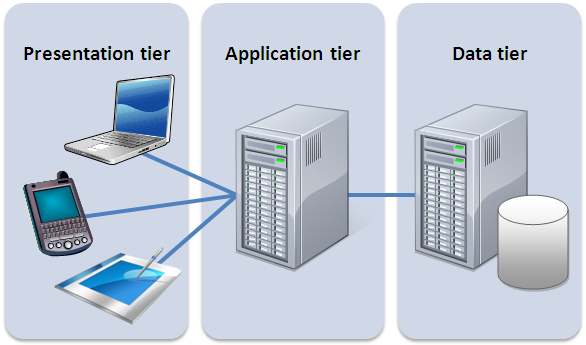
\includegraphics[scale=0.5]{../"Analysis Documents"/3-tier-architecture.png}
	\label{fig:3-tier-architecture}
	\caption{An example of three-tier-architecture}
\end{figure}
\paragraph{} So we subdivide our system in three extremely separated layers (or \textit{tiers}):
\begin{itemize}
	\item A \textit{presentation} layer for the graphic rendering of the data and events generated by the system, and from which the end user can interact with the system
	\item An \textit{application} layer entitled to manage all the business logic of the system
	\item A \textit{Data} layer responsible of the storage of informations to be used by the application and presentation layer
\end{itemize}
The three levels are completely independent and can be replaced easily. In particular, the presentation layer cannot communicate directly with the data tier, but it must forward its requests to the application one, which will use some data access framework to access the database.
\subsection{An overview of our system}
In the specific case of \textit{myTaxiService} we mapped the previous architecture in this way:
\begin{itemize}
	\item \textbf{Presentation tier}:
	\begin{itemize}
		\item \textit{Passenger}:
		\begin{itemize}
			\item Dedicated Mobile application
			\item Browser
		\end{itemize}
		\item \textit{Taxi Driver}:
		\begin{itemize}
			\item Dedicated Mobile application
		\end{itemize}
	\end{itemize}
	\item \textbf{Application tier}: main server(s) located in some office of the government of the city or (better), a virtual server hosted by some expert company and accessed through the Internet.
	\item \textbf{Data tier}: main database(s) located in some office of the government of the city or (better), a virtual database hosted by some expert company and accessed through the Internet. 
\end{itemize}
